\documentclass[twoside]{book}

% Packages required by doxygen
\usepackage{fixltx2e}
\usepackage{calc}
\usepackage{doxygen}
\usepackage[export]{adjustbox} % also loads graphicx
\usepackage{graphicx}
\usepackage[utf8]{inputenc}
\usepackage{makeidx}
\usepackage{multicol}
\usepackage{multirow}
\PassOptionsToPackage{warn}{textcomp}
\usepackage{textcomp}
\usepackage[nointegrals]{wasysym}
\usepackage[table]{xcolor}

% Font selection
\usepackage[T1]{fontenc}
\usepackage[scaled=.90]{helvet}
\usepackage{courier}
\usepackage{amssymb}
\usepackage{sectsty}
\renewcommand{\familydefault}{\sfdefault}
\allsectionsfont{%
  \fontseries{bc}\selectfont%
  \color{darkgray}%
}
\renewcommand{\DoxyLabelFont}{%
  \fontseries{bc}\selectfont%
  \color{darkgray}%
}
\newcommand{\+}{\discretionary{\mbox{\scriptsize$\hookleftarrow$}}{}{}}

% Page & text layout
\usepackage{geometry}
\geometry{%
  a4paper,%
  top=2.5cm,%
  bottom=2.5cm,%
  left=2.5cm,%
  right=2.5cm%
}
\tolerance=750
\hfuzz=15pt
\hbadness=750
\setlength{\emergencystretch}{15pt}
\setlength{\parindent}{0cm}
\setlength{\parskip}{3ex plus 2ex minus 2ex}
\makeatletter
\renewcommand{\paragraph}{%
  \@startsection{paragraph}{4}{0ex}{-1.0ex}{1.0ex}{%
    \normalfont\normalsize\bfseries\SS@parafont%
  }%
}
\renewcommand{\subparagraph}{%
  \@startsection{subparagraph}{5}{0ex}{-1.0ex}{1.0ex}{%
    \normalfont\normalsize\bfseries\SS@subparafont%
  }%
}
\makeatother

% Headers & footers
\usepackage{fancyhdr}
\pagestyle{fancyplain}
\fancyhead[LE]{\fancyplain{}{\bfseries\thepage}}
\fancyhead[CE]{\fancyplain{}{}}
\fancyhead[RE]{\fancyplain{}{\bfseries\leftmark}}
\fancyhead[LO]{\fancyplain{}{\bfseries\rightmark}}
\fancyhead[CO]{\fancyplain{}{}}
\fancyhead[RO]{\fancyplain{}{\bfseries\thepage}}
\fancyfoot[LE]{\fancyplain{}{}}
\fancyfoot[CE]{\fancyplain{}{}}
\fancyfoot[RE]{\fancyplain{}{\bfseries\scriptsize Generated by Doxygen }}
\fancyfoot[LO]{\fancyplain{}{\bfseries\scriptsize Generated by Doxygen }}
\fancyfoot[CO]{\fancyplain{}{}}
\fancyfoot[RO]{\fancyplain{}{}}
\renewcommand{\footrulewidth}{0.4pt}
\renewcommand{\chaptermark}[1]{%
  \markboth{#1}{}%
}
\renewcommand{\sectionmark}[1]{%
  \markright{\thesection\ #1}%
}

% Indices & bibliography
\usepackage{natbib}
\usepackage[titles]{tocloft}
\setcounter{tocdepth}{3}
\setcounter{secnumdepth}{5}
\makeindex

% Hyperlinks (required, but should be loaded last)
\usepackage{ifpdf}
\ifpdf
  \usepackage[pdftex,pagebackref=true]{hyperref}
\else
  \usepackage[ps2pdf,pagebackref=true]{hyperref}
\fi
\hypersetup{%
  colorlinks=true,%
  linkcolor=blue,%
  citecolor=blue,%
  unicode%
}

% Custom commands
\newcommand{\clearemptydoublepage}{%
  \newpage{\pagestyle{empty}\cleardoublepage}%
}

\usepackage{caption}
\captionsetup{labelsep=space,justification=centering,font={bf},singlelinecheck=off,skip=4pt,position=top}

%===== C O N T E N T S =====

\begin{document}

% Titlepage & ToC
\hypersetup{pageanchor=false,
             bookmarksnumbered=true,
             pdfencoding=unicode
            }
\pagenumbering{alph}
\begin{titlepage}
\vspace*{7cm}
\begin{center}%
{\Large E\+X\+Ception \\[1ex]\large 1.\+0 }\\
\vspace*{1cm}
{\large Generated by Doxygen 1.8.13}\\
\end{center}
\end{titlepage}
\clearemptydoublepage
\pagenumbering{roman}
\tableofcontents
\clearemptydoublepage
\pagenumbering{arabic}
\hypersetup{pageanchor=true}

%--- Begin generated contents ---
\chapter{Data Structure Index}
\section{Data Structures}
Here are the data structures with brief descriptions\+:\begin{DoxyCompactList}
\item\contentsline{section}{\hyperlink{classVector_3_01bool_01_4_1_1BoolReference}{Vector$<$ bool $>$\+::\+Bool\+Reference} }{\pageref{classVector_3_01bool_01_4_1_1BoolReference}}{}
\item\contentsline{section}{\hyperlink{classVector}{Vector$<$ data $>$} \\*Type \hyperlink{classVector}{Vector}. Effective in speed, but spends a lot of memory }{\pageref{classVector}}{}
\item\contentsline{section}{\hyperlink{classVector_3_01bool_01_4}{Vector$<$ bool $>$} \\*Type \hyperlink{classVector_3_01bool_01_4}{Vector$<$bool$>$}. Effective in speed, but spends a lot of memory }{\pageref{classVector_3_01bool_01_4}}{}
\end{DoxyCompactList}

\chapter{File Index}
\section{File List}
Here is a list of all documented files with brief descriptions\+:\begin{DoxyCompactList}
\item\contentsline{section}{\hyperlink{den__exception_8cpp}{den\+\_\+exception.\+cpp} \\*Special exception class }{\pageref{den__exception_8cpp}}{}
\item\contentsline{section}{\hyperlink{main_8cpp}{main.\+cpp} \\*Some example of \hyperlink{classDenException}{Den\+Exception} }{\pageref{main_8cpp}}{}
\end{DoxyCompactList}

\chapter{Data Structure Documentation}
\hypertarget{classDenException}{}\section{Den\+Exception Class Reference}
\label{classDenException}\index{Den\+Exception@{Den\+Exception}}


Special exception class. Displays more information than the standard class.  


\subsection*{Public Types}
\begin{DoxyCompactItemize}
\item 
\mbox{\Hypertarget{classDenException_a3d37ff4dd20ed1e4f83a4b15bea110a1}\label{classDenException_a3d37ff4dd20ed1e4f83a4b15bea110a1}} 
enum {\bfseries exception\+\_\+code\+\_\+e} \{ \newline
{\bfseries U\+N\+T\+I\+T\+L\+ED} = 0, 
{\bfseries D\+I\+V\+\_\+\+B\+Y\+\_\+\+Z\+E\+RO} = 1, 
{\bfseries C\+A\+N\+T\+\_\+\+O\+P\+E\+N\+\_\+\+F\+I\+LE} = 2, 
{\bfseries C\+A\+N\+T\+\_\+\+C\+L\+O\+S\+E\+\_\+\+F\+I\+LE} = 3, 
\newline
{\bfseries A\+R\+R\+A\+Y\+\_\+\+O\+U\+T\+\_\+\+O\+F\+\_\+\+R\+A\+N\+GE} = 4, 
{\bfseries N\+U\+L\+L\+\_\+\+P\+O\+I\+N\+T\+ER} = 5, 
{\bfseries D\+O\+N\+T\+\_\+\+H\+A\+V\+E\+\_\+\+M\+E\+M\+O\+RY} = 6
 \}
\end{DoxyCompactItemize}
\subsection*{Public Member Functions}
\begin{DoxyCompactItemize}
\item 
\hyperlink{classDenException_a126de088ce459641b0793bd754f4d171}{Den\+Exception} (const char $\ast$filename, const char $\ast$func, const long int line, const char $\ast$message, exception\+\_\+code\+\_\+e exc\+\_\+code)
\begin{DoxyCompactList}\small\item\em constructor  create a \hyperlink{classDenException}{Den\+Exception} \end{DoxyCompactList}\item 
\hyperlink{classDenException_a515eeb5f86c2ed600a484b2653b10e48}{Den\+Exception} (const \hyperlink{classDenException}{Den\+Exception} \&except)
\begin{DoxyCompactList}\small\item\em copy constructor  deeply copies one \hyperlink{classDenException}{Den\+Exception} to another \end{DoxyCompactList}\item 
\hyperlink{classDenException_a6e21462a638a18d3af11e183bbb2e441}{Den\+Exception} (\hyperlink{classDenException}{Den\+Exception} \&\&except)
\begin{DoxyCompactList}\small\item\em move constructor  superficially copies the temporary vector \end{DoxyCompactList}\item 
\mbox{\Hypertarget{classDenException_a90812cb3af8ed4794c411b575c30c5c0}\label{classDenException_a90812cb3af8ed4794c411b575c30c5c0}} 
\hyperlink{classDenException_a90812cb3af8ed4794c411b575c30c5c0}{$\sim$\+Den\+Exception} (void)
\begin{DoxyCompactList}\small\item\em destructor  free Vector \end{DoxyCompactList}\item 
void \hyperlink{classDenException_a9ea40d7917b2148f9183ce63bde612a8}{where} (std\+::ostream \&os)
\begin{DoxyCompactList}\small\item\em displays the location of \hyperlink{classDenException}{Den\+Exception} \end{DoxyCompactList}\item 
void \hyperlink{classDenException_a52785aeb451bf203cda123c8dcc9d64e}{what} (std\+::ostream \&os)
\begin{DoxyCompactList}\small\item\em displays an exception message \end{DoxyCompactList}\item 
void \hyperlink{classDenException_a81eaeb9c2f6845516f25ead861040a93}{code} (std\+::ostream \&os)
\begin{DoxyCompactList}\small\item\em displays an exception code \end{DoxyCompactList}\end{DoxyCompactItemize}
\subsection*{Private Attributes}
\begin{DoxyCompactItemize}
\item 
\mbox{\Hypertarget{classDenException_ac00d70d94b80bee04c3bd1001dcb9b59}\label{classDenException_ac00d70d94b80bee04c3bd1001dcb9b59}} 
char $\ast$ {\bfseries message\+\_\+}
\item 
\mbox{\Hypertarget{classDenException_a208f77c9eef3ca77c9856d53d61f6521}\label{classDenException_a208f77c9eef3ca77c9856d53d61f6521}} 
exception\+\_\+code\+\_\+e {\bfseries exc\+\_\+code\+\_\+}
\item 
\mbox{\Hypertarget{classDenException_af1a100cc67470e358b9f372cbc157830}\label{classDenException_af1a100cc67470e358b9f372cbc157830}} 
char $\ast$ {\bfseries filename\+\_\+}
\item 
\mbox{\Hypertarget{classDenException_abbaa230a9b0fe68e0ef7eaad171f79a4}\label{classDenException_abbaa230a9b0fe68e0ef7eaad171f79a4}} 
char $\ast$ {\bfseries func\+\_\+}
\item 
\mbox{\Hypertarget{classDenException_a5b7be04f7a34c9944e0d0e934e88ef26}\label{classDenException_a5b7be04f7a34c9944e0d0e934e88ef26}} 
long int {\bfseries line\+\_\+}
\end{DoxyCompactItemize}


\subsection{Detailed Description}
Special exception class. Displays more information than the standard class. 

Definition at line 21 of file den\+\_\+exception.\+cpp.



\subsection{Constructor \& Destructor Documentation}
\mbox{\Hypertarget{classDenException_a126de088ce459641b0793bd754f4d171}\label{classDenException_a126de088ce459641b0793bd754f4d171}} 
\index{Den\+Exception@{Den\+Exception}!Den\+Exception@{Den\+Exception}}
\index{Den\+Exception@{Den\+Exception}!Den\+Exception@{Den\+Exception}}
\subsubsection{\texorpdfstring{Den\+Exception()}{DenException()}\hspace{0.1cm}{\footnotesize\ttfamily [1/3]}}
{\footnotesize\ttfamily Den\+Exception\+::\+Den\+Exception (\begin{DoxyParamCaption}\item[{const char $\ast$}]{filename,  }\item[{const char $\ast$}]{func,  }\item[{const long int}]{line,  }\item[{const char $\ast$}]{message = {\ttfamily NULL},  }\item[{exception\+\_\+code\+\_\+e}]{exc\+\_\+code = {\ttfamily UNTITLED} }\end{DoxyParamCaption})}



constructor  create a \hyperlink{classDenException}{Den\+Exception} 


\begin{DoxyParams}[1]{Parameters}
\mbox{\tt in}  & {\em filename} & \\
\hline
\mbox{\tt in}  & {\em func} & \\
\hline
\mbox{\tt in}  & {\em line} & \\
\hline
\mbox{\tt in}  & {\em message} & \\
\hline
\mbox{\tt in}  & {\em exc\+\_\+code} & \\
\hline
\end{DoxyParams}


Definition at line 67 of file den\+\_\+exception.\+cpp.


\begin{DoxyCode}
68   \{
69     filename\_ = strdup(filename);
70     func\_     = strdup(func);
71     line\_     = line;
72 
73     exc\_code\_ = exc\_code;
74     message\_  = strdup(message);
75   \}
\end{DoxyCode}
\mbox{\Hypertarget{classDenException_a515eeb5f86c2ed600a484b2653b10e48}\label{classDenException_a515eeb5f86c2ed600a484b2653b10e48}} 
\index{Den\+Exception@{Den\+Exception}!Den\+Exception@{Den\+Exception}}
\index{Den\+Exception@{Den\+Exception}!Den\+Exception@{Den\+Exception}}
\subsubsection{\texorpdfstring{Den\+Exception()}{DenException()}\hspace{0.1cm}{\footnotesize\ttfamily [2/3]}}
{\footnotesize\ttfamily Den\+Exception\+::\+Den\+Exception (\begin{DoxyParamCaption}\item[{const \hyperlink{classDenException}{Den\+Exception} \&}]{except }\end{DoxyParamCaption})}



copy constructor  deeply copies one \hyperlink{classDenException}{Den\+Exception} to another 


\begin{DoxyParams}[1]{Parameters}
\mbox{\tt in}  & {\em \hyperlink{classDenException}{Den\+Exception}} & copy \hyperlink{classDenException}{Den\+Exception} \\
\hline
\end{DoxyParams}


Definition at line 82 of file den\+\_\+exception.\+cpp.


\begin{DoxyCode}
83   \{
84     filename\_ = strdup(except.filename\_);
85     func\_     = strdup(except.func\_);
86     line\_     = except.line\_;
87 
88     exc\_code\_ = except.exc\_code\_;
89     message\_  = strdup(except.message\_);
90   \}
\end{DoxyCode}
\mbox{\Hypertarget{classDenException_a6e21462a638a18d3af11e183bbb2e441}\label{classDenException_a6e21462a638a18d3af11e183bbb2e441}} 
\index{Den\+Exception@{Den\+Exception}!Den\+Exception@{Den\+Exception}}
\index{Den\+Exception@{Den\+Exception}!Den\+Exception@{Den\+Exception}}
\subsubsection{\texorpdfstring{Den\+Exception()}{DenException()}\hspace{0.1cm}{\footnotesize\ttfamily [3/3]}}
{\footnotesize\ttfamily Den\+Exception\+::\+Den\+Exception (\begin{DoxyParamCaption}\item[{\hyperlink{classDenException}{Den\+Exception} \&\&}]{except }\end{DoxyParamCaption})}



move constructor  superficially copies the temporary vector 


\begin{DoxyParams}[1]{Parameters}
\mbox{\tt in}  & {\em Vector} & copy Vector \\
\hline
\end{DoxyParams}


Definition at line 97 of file den\+\_\+exception.\+cpp.


\begin{DoxyCode}
98   \{
99     filename\_ = except.filename\_;
100     func\_     = except.func\_;
101     line\_     = except.line\_;
102 
103     exc\_code\_ = except.exc\_code\_;
104     message\_  = except.message\_;
105   \}
\end{DoxyCode}


\subsection{Member Function Documentation}
\mbox{\Hypertarget{classDenException_a81eaeb9c2f6845516f25ead861040a93}\label{classDenException_a81eaeb9c2f6845516f25ead861040a93}} 
\index{Den\+Exception@{Den\+Exception}!code@{code}}
\index{code@{code}!Den\+Exception@{Den\+Exception}}
\subsubsection{\texorpdfstring{code()}{code()}}
{\footnotesize\ttfamily void Den\+Exception\+::code (\begin{DoxyParamCaption}\item[{std\+::ostream \&}]{os }\end{DoxyParamCaption})}



displays an exception code 


\begin{DoxyParams}[1]{Parameters}
\mbox{\tt in}  & {\em os} & output stream \\
\hline
\end{DoxyParams}


Definition at line 150 of file den\+\_\+exception.\+cpp.


\begin{DoxyCode}
151   \{
152     os << \textcolor{stringliteral}{"code error: "} << exc\_code\_ << std::endl;
153   \}
\end{DoxyCode}
\mbox{\Hypertarget{classDenException_a52785aeb451bf203cda123c8dcc9d64e}\label{classDenException_a52785aeb451bf203cda123c8dcc9d64e}} 
\index{Den\+Exception@{Den\+Exception}!what@{what}}
\index{what@{what}!Den\+Exception@{Den\+Exception}}
\subsubsection{\texorpdfstring{what()}{what()}}
{\footnotesize\ttfamily void Den\+Exception\+::what (\begin{DoxyParamCaption}\item[{std\+::ostream \&}]{os }\end{DoxyParamCaption})}



displays an exception message 


\begin{DoxyParams}[1]{Parameters}
\mbox{\tt in}  & {\em os} & output stream \\
\hline
\end{DoxyParams}


Definition at line 138 of file den\+\_\+exception.\+cpp.


\begin{DoxyCode}
139   \{
140     \textcolor{keywordflow}{if}(message\_ != NULL)
141       os << message\_ << std::endl;
142     \textcolor{keywordflow}{else}
143       os << \textcolor{stringliteral}{"message is null"} << std::endl;
144   \}
\end{DoxyCode}
\mbox{\Hypertarget{classDenException_a9ea40d7917b2148f9183ce63bde612a8}\label{classDenException_a9ea40d7917b2148f9183ce63bde612a8}} 
\index{Den\+Exception@{Den\+Exception}!where@{where}}
\index{where@{where}!Den\+Exception@{Den\+Exception}}
\subsubsection{\texorpdfstring{where()}{where()}}
{\footnotesize\ttfamily void Den\+Exception\+::where (\begin{DoxyParamCaption}\item[{std\+::ostream \&}]{os }\end{DoxyParamCaption})}



displays the location of \hyperlink{classDenException}{Den\+Exception} 


\begin{DoxyParams}[1]{Parameters}
\mbox{\tt in}  & {\em os} & output stream \\
\hline
\end{DoxyParams}


Definition at line 129 of file den\+\_\+exception.\+cpp.


\begin{DoxyCode}
130   \{
131     os << \textcolor{stringliteral}{"file: "} << filename\_ << \textcolor{stringliteral}{", function: "} << func\_ << \textcolor{stringliteral}{", line: "} << line\_ << std::endl;
132   \}
\end{DoxyCode}


The documentation for this class was generated from the following file\+:\begin{DoxyCompactItemize}
\item 
\hyperlink{den__exception_8cpp}{den\+\_\+exception.\+cpp}\end{DoxyCompactItemize}

\chapter{File Documentation}
\hypertarget{den__exception_8cpp}{}\section{den\+\_\+exception.\+cpp File Reference}
\label{den__exception_8cpp}\index{den\+\_\+exception.\+cpp@{den\+\_\+exception.\+cpp}}


special exception class  


{\ttfamily \#include $<$iostream$>$}\newline
{\ttfamily \#include $<$fstream$>$}\newline
{\ttfamily \#include $<$string.\+h$>$}\newline
Include dependency graph for den\+\_\+exception.\+cpp\+:\nopagebreak
\begin{figure}[H]
\begin{center}
\leavevmode
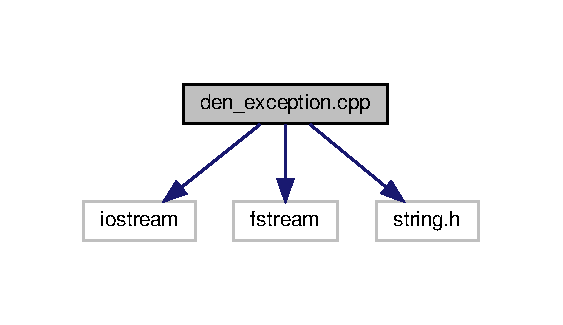
\includegraphics[width=270pt]{den__exception_8cpp__incl}
\end{center}
\end{figure}
This graph shows which files directly or indirectly include this file\+:\nopagebreak
\begin{figure}[H]
\begin{center}
\leavevmode
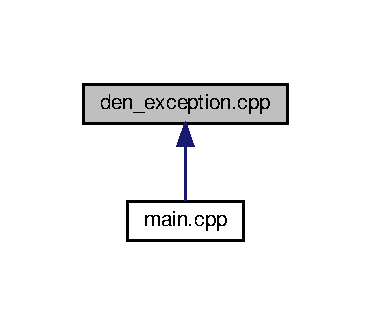
\includegraphics[width=178pt]{den__exception_8cpp__dep__incl}
\end{center}
\end{figure}
\subsection*{Data Structures}
\begin{DoxyCompactItemize}
\item 
class \hyperlink{classDenException}{Den\+Exception}
\begin{DoxyCompactList}\small\item\em Special exception class. Displays more information than the standard class. \end{DoxyCompactList}\end{DoxyCompactItemize}


\subsection{Detailed Description}
special exception class 

\begin{DoxyAuthor}{Author}
Den 
\end{DoxyAuthor}
\begin{DoxyVersion}{Version}
1.\+0 
\end{DoxyVersion}
\begin{DoxyDate}{Date}
March 2019 
\end{DoxyDate}

\hypertarget{main_8cpp}{}\section{main.\+cpp File Reference}
\label{main_8cpp}\index{main.\+cpp@{main.\+cpp}}


some example of \hyperlink{classVector}{Vector}  


{\ttfamily \#include \char`\"{}vector.\+cpp\char`\"{}}\newline
Include dependency graph for main.\+cpp\+:
\nopagebreak
\begin{figure}[H]
\begin{center}
\leavevmode
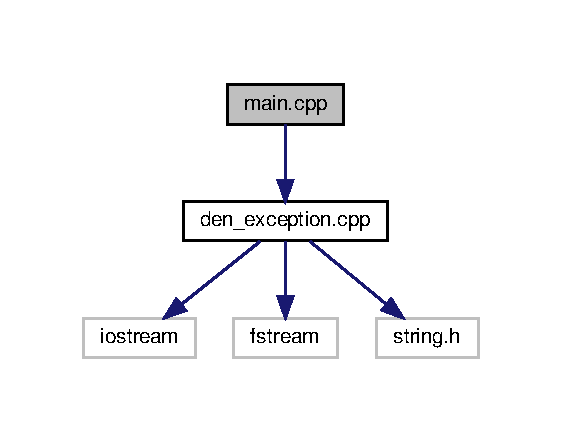
\includegraphics[width=350pt]{main_8cpp__incl}
\end{center}
\end{figure}
\subsection*{Functions}
\begin{DoxyCompactItemize}
\item 
\mbox{\Hypertarget{main_8cpp_a840291bc02cba5474a4cb46a9b9566fe}\label{main_8cpp_a840291bc02cba5474a4cb46a9b9566fe}} 
int {\bfseries main} (void)
\end{DoxyCompactItemize}


\subsection{Detailed Description}
some example of \hyperlink{classVector}{Vector} 

\begin{DoxyAuthor}{Author}
Den 
\end{DoxyAuthor}
\begin{DoxyVersion}{Version}
1.\+0 
\end{DoxyVersion}
\begin{DoxyDate}{Date}
March 2019 
\end{DoxyDate}

%--- End generated contents ---

% Index
\backmatter
\newpage
\phantomsection
\clearemptydoublepage
\addcontentsline{toc}{chapter}{Index}
\printindex

\end{document}
